\documentclass[10pt]{article}
\usepackage{tikz}
\usepackage[pdf]{graphviz}

\begin{document}
\title{Tugas 1 : Rangkuman Pemodelan Pertemuan 1}
\author{Donny Prakarsa Utama\\3332170032\\Pemodelan dan Indentifikasi Sistem-1}
\date{March 30, 2021}
\maketitle

\section{Pemodelan}
Mampu melakukan analisis dan pembuatan model sistem keelektronikaan, mempelajari pemilihan dan penerapan model dan simulasi sistem keelektronikaan, pemodelan matematis, analisa spektrum, time-series model, waktu kontinyu dan Indentifikasi sistem. 
\section{Sistem}
Sistem adalah kumpulan elemen yang bekerjasama mencapai tujuan yang diharapkan. Sistem terdiri dari berbagai elemen yang membentuk satu kesatuan. Adanya interaksi saling ketergantungan dan kerjasama antarelemen. Sistem mencapai tujuan tertentu. Sistem miliki mekanisme dan lingkungan serta dinamika sistem.\\ \textbf{Elemen} adalah bagian dasar sistem yang mebentuk sistem tersebut.\\ \textbf{Atribut} adalah sifat atau perwujudan yang dapat dilihat dari elemen. \\ \textbf{Relasi} adalah keterkaitan antar elemen dan atribut.
\begin{figure}
\centering
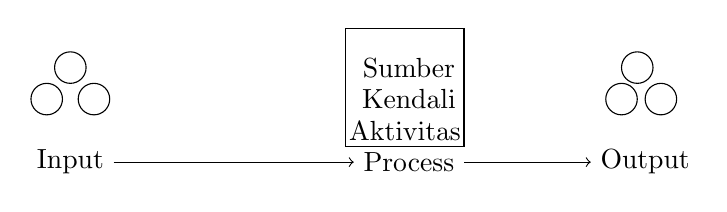
\begin{tikzpicture}
\node (B)at(4.8,-0.2){Process};
\node(A) at (0.5,-0.2) {Input};
\node (C) at (7.8,-0.2){Output};
\node (b3) at (4.8,1){Sumber};
\node (b1) at (4.8,0.6){Kendali};
\node (b2) at (4.75,0.2){Aktivitas};
\draw (0.5,1) circle (0.2) ;
\draw (0.2,0.6) circle (0.2) ;
\draw (0.8,0.6) circle (0.2) ;
\draw (7.7,1) circle (0.2) ;
\draw (7.5,0.6) circle (0.2) ;
\draw (8,0.6) circle (0.2) ;
\draw (4,0) rectangle (5.5,1.5);
\draw[->](A) -> (B);
\draw[->](B) -> (C);
\end{tikzpicture}
\caption{Model Sistem Sederhana}
\label{fig:1}
\end{figure}

Misal pada \figurename{\ref{fig:1}} sistem terdiri dari input, proses dan output. Dalam contoh kendali suhu, elemen adalah berupa pemanas, sensor pengukur panas. Atributnya adalah suhu udara. Relasi adalah keterkaitan antara elemen baik pada sistem yang dibuat maupun diluar hal itu. 
Misalnya $f(T^{\circ}Ruangan)=f(T^{\circ}AC)+f(T^{\circ}Kipas)-f(T^{\circ}Suhu tubuh)$
\section{Subsistem}
Sistem terdiri dari subsistem atau elemen-elemen yang menyusun suatu sistem. Misalnya dalam Sistem Kelistrikan pada Industri. Subsistem terdiri dari ruang kendali, ruang pendinginan, ruang instrumentasi, generator listrik, gardu listrik dsb.
\begin{figure}[!t]
    \centering
\digraph[scale=0.7]{D} {
    node[shape="rectangle"]
    { rank=same; c b };
    { rank=same; d e };
a[label="Sistem"]
b[label="Subsistem A"]
c[label="Subsistem B"]
d[label="Elemen 1"]
e[label="Elemen 2"]
a->c,b 
b->d,e
}
\caption{Subsistem}
\label{fig:2}
\end{figure}

\section{Lingkungan}
Lingkungan adalah segala sesutau yang diluar sistem. Misalkan sistem pendingin ruangan, maka lingkungan adalah suhu panas dari dalam atau luar ruangan (suhu tubuh, suhu sinar matahari dsb).
Dalam merancang sistem terhadap pengaruh lingkungan, ada 2 jenis sistem yaitu sistem terbuka dan sistem tertutup. Sistem terbuka adalah sistem yang tidak dipengaruhi oleh lingkungan sedangkan sistem terbuka dipengaruhi oleh lingkungan.
Pada \figurename{\ref{fig:1}} input bisa jadi sebuah lingkungan yang mempengaruhi sistem dan output merupakan hasil dari sistem yang mempengaruhi lingkungan.
\section{Pemodelan Sistem}
Cara untuk melakukan pemodelan sistem adalah menentukan karakteristik fisik dari yang ingin dimodelkan. kemudian dibuat kedalam persamaan matemaatis.
Keuntungan menggunakan model:
\begin{itemize}
    \item Hemat biaya
    \item Hemat waktu
    \item Dapat melakukan percobaan
    \item Fokus pada karakteristik permasalahan
\end{itemize}
Dengan model, kita dapat melakukan simulasi terhadap sistem.
\section{Simulasi}
Simulasi adalah tiruan dari sebuah sistem dinamis dengan menggunakan model komputer untuk melakukan evaluasi kerja meningkatkan kinerja sistem.
\subsection{Why?}
\begin{itemize}
    \item Simulasi bagaikan dukun yang dapat melakukan peramalan dari suatu kinerja sistem, bahkan yang paling rumit
    \item Decision making, Try and Error.
\end{itemize}

\end{document}